\documentclass[14pt]{extreport}
\usepackage{gost}
\usepackage{tikz}
\usepackage{listings}
\usetikzlibrary{shapes.geometric}
\begin{document}
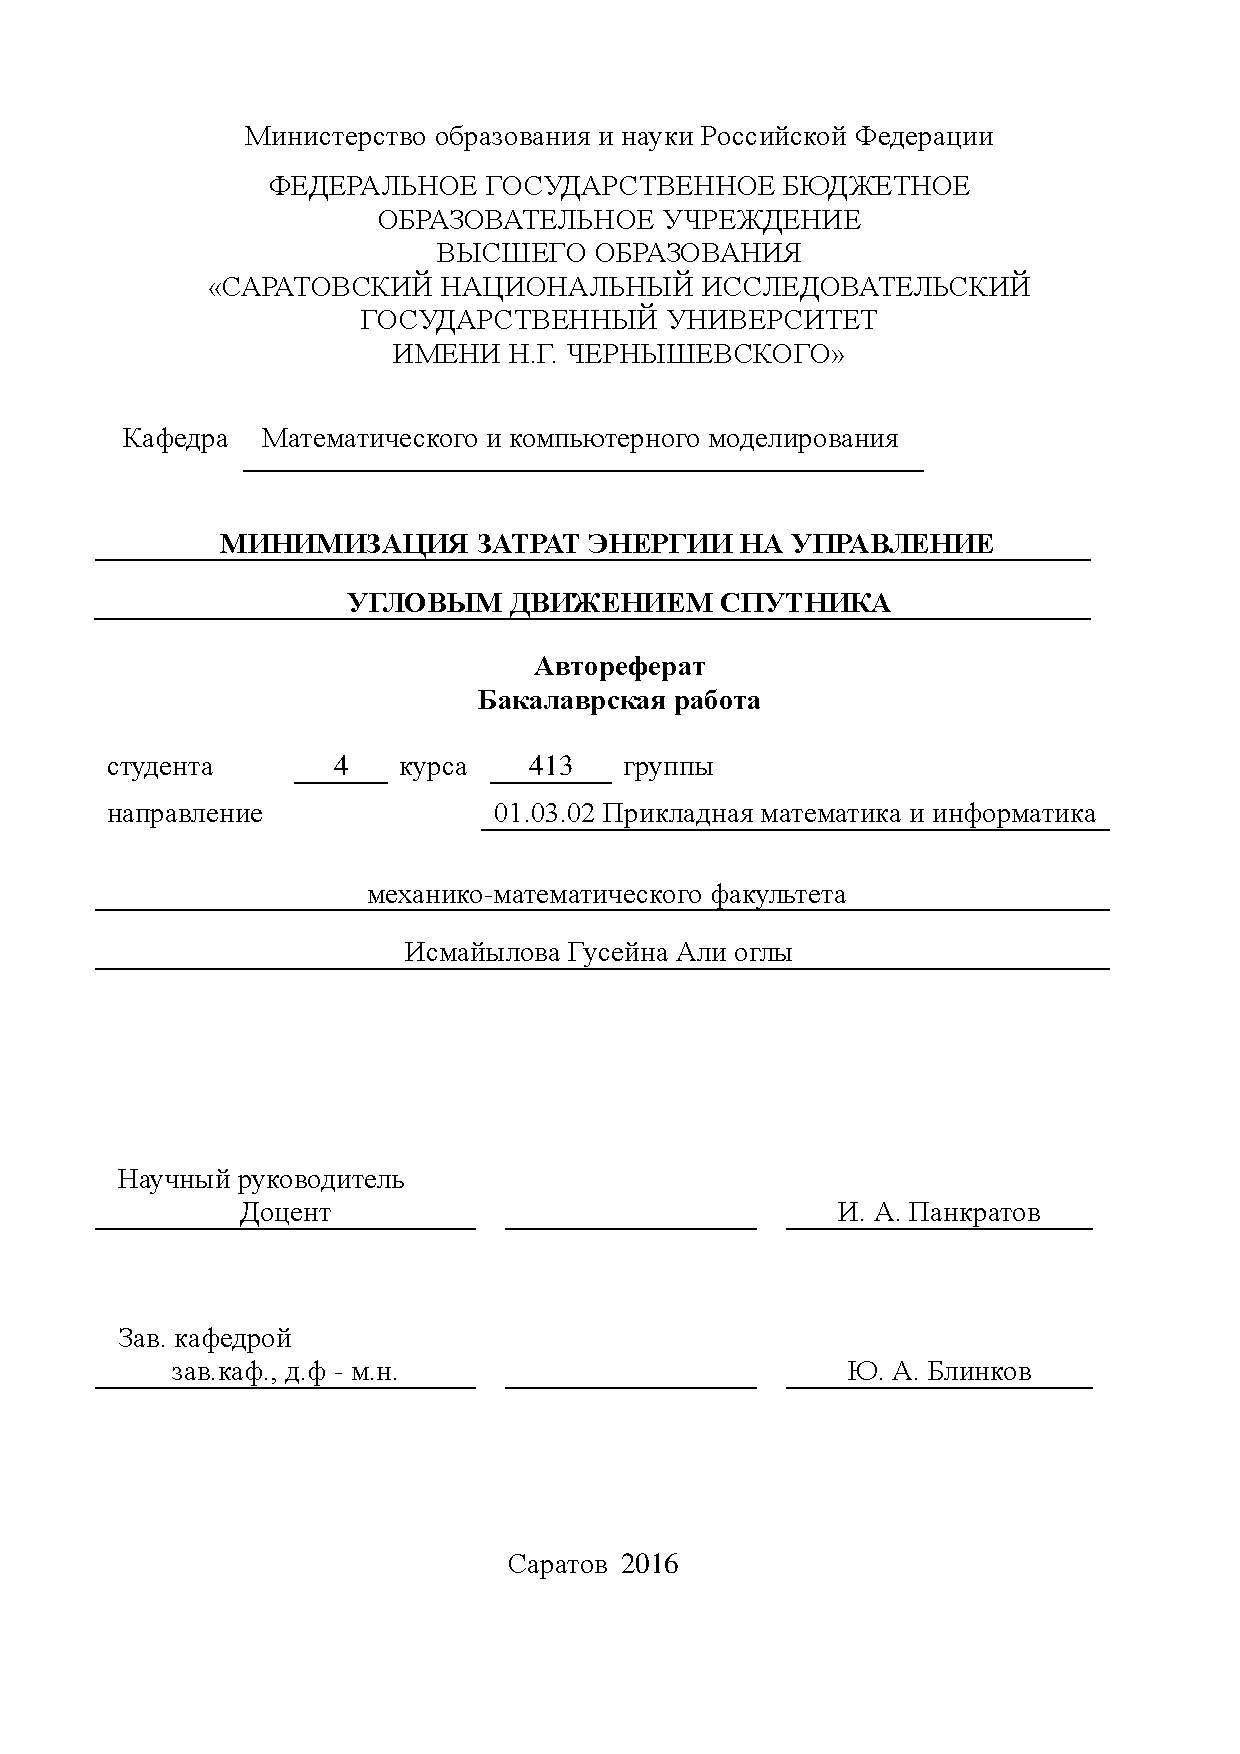
\includepdf[pages={1}]{titulRef.pdf}

\tableofcontents

\intro

Представленная квалификационная работа посвящена разработке методов решения задач оптимального управления для углового движения спутника.
Такие задачи составляют активно исследуемое направление прикладной математики.
Особое внимание в работе уделено исследованию достаточных условий оптимальности в
принципе максимума Понтрягина. Основные результаты связаны с разработкой алгоритмов построения оптимальных траекторий и оптимальных управлений. 

Необходимо рассмотреть случай минимизации энергии на перевод искусственного спутника Земли в нужное угловое положение.
Время окончания процесса фиксировано. Также требуется рассмотреть задачу с её различными параметрами и вывести основные закономерности.

\chapter{Общая характеристика работы}

\section{Актуальность работы}

Теория управления является в настоящее время быстро развивающимся разделом современной математики, что
вызвано потребностями многочисленных приложений в таких разнообразных
дисциплинах как аэрокосмические науки, инженерные и технические науки, гибридные
системы, вычислительные и
компьютерные науки, океанографические, физические и математические науки. Возрастает интерес к теории оптимального управления
и ее приложениям у математиков, экономистов и специалистов по проблемам окружающей среды, а также международных научных организаций, что
подтверждается увеличением количества работ в российских и зарубежных издательствах.

\section{Цели и задачи работы}

Цель работы заключается в исследовании свойств оптимальных решений в
задачах управления угловым движением спутника при разлиных параметрах, изучении достаточных условий оптимальности в принципе максимума Понтрягина,
разработке алгоритмов построения оптимальных траекторий и оптимальных управлений. Также необходимо автоматизировать все используюемые для решения алгоритмы программным образом.

В данной работе будут представлены основные определения, понятния и теоремы, которые позволят составить и решить поставленную задачу,
решение которой состоит из двух частей: аналитической и численной. Аналитическая часть позволяет перевести задачу оптимального управления
к краевой задаче, для которой составляется алгоритм в численной части. Для реализации такого алгоритма будет написана программа,
которая будет выдавать результаты решения краевой задачи, а также генерировать скрипт для графиков, которые наглядным образом будут отражать
суть этих результатов.


\section{Научная новизна}

Научая новизна данной работы состоит в рассмотрении поставленной задачи с применением алгебры кватернионов не только в теоритических выкладках,
но и в программной реализации решения, которая является универсальной для любого типа задач управления благодаря использованию интерфейсов
в программе, которые могут быть ипользованы для самых различных уравнений состояния.

\section{Достоверность полученных результатов}

Достоверность полученных результатов следуюет из разбора многочисленных случаев решения задачи для разных параметров и сравнивания их
с очевидными свойствами функционала качества управления.

\section{Практическая значимость работы}

Полученные в работе теоритические результаты позволяют понять основные зависимости функционала качества управления и его параметров,
а также прогнозировать поведение системы при изменениях параметров самой задачи. Более того, написанные программы позволяют в общем случае рассматривать любую задачу управления.

\chapter{Содержание выпускной квалификационной работы}

\section{Постановка задачи}

Пусть угловое движение тела описывается кинематическим уравнением Пуассона

\begin{equation}
2\dot{\Lambda}\ =\ \Lambda \circ \Omega,
\end{equation}
где $\Lambda\ =\ \Lambda(\lambda_0,\ (\lambda_1,\ \lambda_2,\ \lambda_3))$ --- кватернион, характеризующий положение твердого тела относительно инерциальной системы координат,
$\Omega\ =\ \Omega(\omega_0,\ (\omega_1,\ \omega_2,\ \omega_3))$ --- кватернион, векторная часть которого равна абсолютной угловой скорости твердого тела относительно этой системы,
а скалярная часть равна нулю.

Выражение $(2.1)$ в развернутом виде выглядит следующим образом

\begin{equation}
\begin{cases}
2\dot{\lambda_0}\ =\ -\lambda_1\omega_1\ -\ \lambda_2\omega_2\ -\ \lambda_3\omega_3, \\
2\dot{\lambda_1}\ =\ \lambda_0\omega_1\ +\ \lambda_2\omega_3\ -\ \lambda_3\omega_2, \\
2\dot{\lambda_2}\ =\ \lambda_0\omega_2\ +\ \lambda_3\omega_1\ -\ \lambda_1\omega_3, \\
2\dot{\lambda_3}\ =\ \lambda_0\omega_3\ +\ \lambda_1\omega_2\ -\ \lambda_2\omega_1.
 \end{cases}
\end{equation}

Также дано начальное угловое положение 

\begin{equation}
\Lambda(0)\ =\ \Lambda^0.
\end{equation}
И конечное угловое положение

\begin{equation}
\Lambda(T)\ =\ \Lambda^T.
\end{equation}

Требуется найти такое оптимальное управление $\Omega(t)$, чтобы функционал качества 

\begin{equation}
I\ =\ \int_{0}^{T}(\alpha_1\omega_1\ +\ \alpha_2\omega_2\ +\ \alpha_3\omega_3)dt,
\end{equation}
где $\alpha_1,\ \alpha_2,\ \alpha_3\ =\ const\ >\ 0$ --- весовые множители функционала $(2.5)$, $\omega_1,\ \omega_2,\ \omega_3$ --- компоненты векторной части $\Omega$,
принимал минимальные значения при фиксированном $T$.

Функционал качества $(2.5)$ характеризует общие энергетические затраты на управление.
Для начала задача будет решена в общем случае, а затем будут рассмотрены конкретные примеры.

\section{Аналитическая часть решения}

Воспользуемся методом максимума Понтрягина, суть которого заключается в том, что задача оптимального управления сводится к решению краевой задачи
для системы обыкновенных дифференциальных уравнений.

Таким образом мы приходим к следующей краевой задаче

\begin{equation}
\begin{cases}
2\dot{\Lambda}\ =\ \Lambda\ \circ\ \Omega, \\
2\dot{\Psi}\ =\ \Psi\ \circ\ \Omega, \\
\Omega\ =\ \bigg(0\ ,\bigg(\dfrac{p_1}{4\alpha_1},\ \dfrac{p_2}{4\alpha_3},\ \dfrac{p_3}{4\alpha_3}\bigg) \bigg), \\
\Lambda(0)\ =\ \Lambda^0, \\
\Lambda(T)\ =\ \Lambda^T,
 \end{cases}
\end{equation}
где 

\begin{equation}
\begin{cases}
p_1\ =\ - \psi_0\lambda_1\ +\ \psi_1\lambda_0\ +\ \psi_2\lambda_3\ -\ \psi_3\lambda_2, \\
p_2\ =\ - \psi_0\lambda_2\ -\ \psi_1\lambda_3\ +\ \psi_2\lambda_0\ +\ \psi_3\lambda_1, \\
p_3\ =\ - \psi_0\lambda_3\ +\ \psi_1\lambda_2\ -\ \psi_2\lambda_1\ +\ \psi_3\lambda_0.
 \end{cases}
\end{equation}

\section{Численная часть решения}

Воспользуемся методом Ньютона для решения краевой задачи $(2.6)$. Суть данного итерационного метода состоит в том, что краевая задача сводится
к решению серии задач Коши при фиксированном начальном условии с помощью некоторого начального приближения параметра,
затем проверяется конечное условие, и если оно удовлетворяется с некоторой требуемой точностью, то задача решена, иначе находится новое приближение,
построенное на предыдущем.

\section{Исследование результатов}


Расмотрим задачу оптимального управления, которой соответствует краевая задача $(2.8)$ для тела, начальное положение которого задано углами Эйлера:
$\alpha\ =\ -78.4^{\circ},\ \beta\ =\ -39.9^{\circ},\ \gamma\ =\ 112.9^{\circ}$,
а конечное --- $\widetilde\alpha\ =\ 0^{\circ},\ \widetilde\beta\ =\ 0^{\circ},\ \widetilde\gamma\ =\ 0^{\circ}$. 
Пусть требуется решить задачу с точностью $\varepsilon = 10^{-9}$ при весовых множителях $\alpha_1 = 1000,\ \alpha_2 = 2000,\ \alpha_3 = 3000$ для времени
$T\ =\ 300c$.

\begin{equation}
\begin{cases}
2\dot{\Lambda}\ =\ \Lambda \circ \Omega,\\
 \Lambda(0)\ =\ \Lambda^{0}(\lambda_0^{0},\ (\lambda_1^{0},\ \lambda_2^{0},\ \lambda_3^{0})), \\
 \lambda_{0}^{0}\ =\ -0.5821271946729387, \\
 \lambda_{1}^{0}\ =\ 0.10821947847990215, \\
 \lambda_{2}^{0}\ =\ 0.641192910029563, \\
 \lambda_{3}^{0}\ =\-0.48814764756943485. \\
 \Lambda(T)\ =\ \Lambda^{T}(\lambda_0^{T},\ (\lambda_1^{T},\ \lambda_2^{T},\ \lambda_3^{T})), \\
 \lambda_{0}^{T}\ =\ 1, \ 
 \lambda_{1}^{T}\ =\ 0, \ 
 \lambda_{2}^{T}\ =\ 0, \ 
 \lambda_{3}^{T}\ =\ 0. \ 
 \end{cases}
\end{equation}

Тогда график изменения компонент кватерниона $\Lambda\ =\ \Lambda(\lambda_0,\ (\lambda_1,\ \lambda_2, \lambda_3))$ с течением времени,
найденное в ходе решения, представлен на рисунке $2.1$, по которому видно, что оптимальное управление переводит тело из заданного начального
углового положения в требуемое конечное.

Найденное решение $\Lambda$ позволяет получить данные об изменениях углов Эйлера, задающие угловое положение тела.
На рисунках $2.2\ -\ 2.4$ представлены изменения углов прецессии, нутации, собственного вращения соответственно.

\begin{center}
\vspace*{50px}
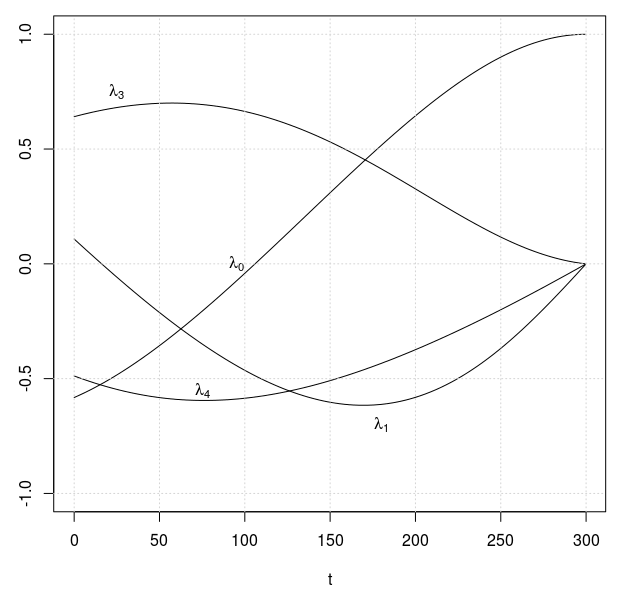
\includegraphics[width=17cm, height=17cm]{l300.png}

Рисунок $2.1$. 
\end{center}

\begin{center}
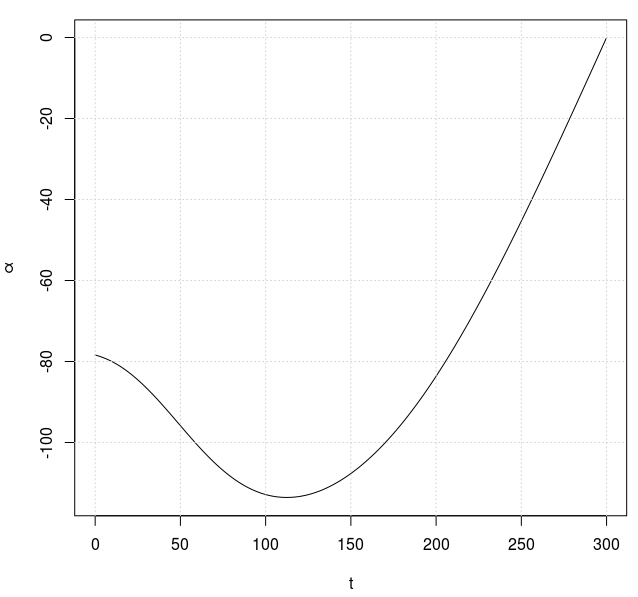
\includegraphics[width=11cm, height=11cm]{alpha.png}

Рисунок $2.2$  --- изменение угла прецессии. 
\end{center}

\begin{center}
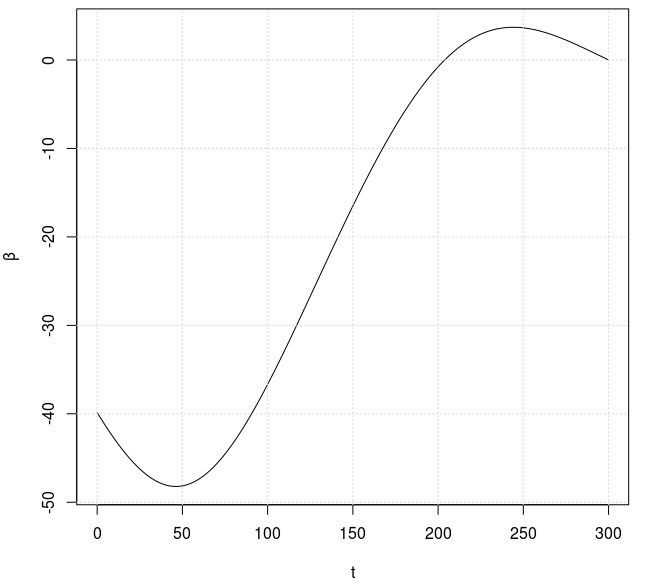
\includegraphics[width=11cm, height=11cm]{beta.png}

Рисунок $2.3$  --- изменение угла прецессии. 
\end{center}

\begin{center}
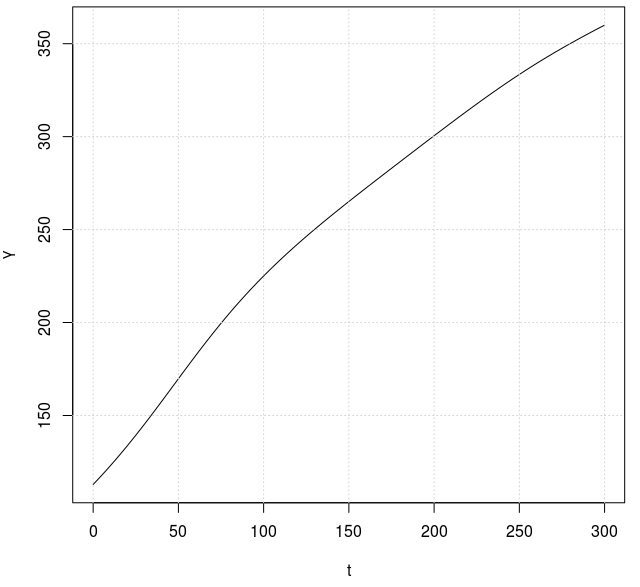
\includegraphics[width=11cm, height=11cm]{gamma.png}

Рисунок $2.4$  --- изменение угла собственного вращения. 
\end{center}

Рисунки $2.2\ -\ 2.4$ полностью соответствуют рисунку $2.1$, и следовательно требованиям для оптимального управления.

В поставленной задаче в качестве оптимального управления, как было сказано ранее, выступает угловая скорость
$\Omega = \Omega(\omega_0,\ (\omega_1,\ \omega_2,\ \omega_3))$, которая также находится в ходе решения краевой задачи $(2.6)$. График изменения
компонент угловой скорости $\omega_1,\ \omega_2,\ \omega_3$ представлен на рисунке $2.5$.

Основная трудность, с которой можно столкнуться при решении задачи оптмального управления для больших углов отклонения между начальным и конечным
положенииями тела --- это нахождение начального приближения $\Psi$, поэтому желательно знать, где приблизительно его можно находить. 

Для данной задачи график изменения компонент кватерниона $\Psi\ =\ \Psi(\psi_0,\ (\psi_1,\ \psi_2, \psi_3))$, который получается на последней итерации
метода Ньютона решения краевой задачи $(2.6)$, представлен на рисунке $2.5$.

\begin{center}
\vspace*{50px}
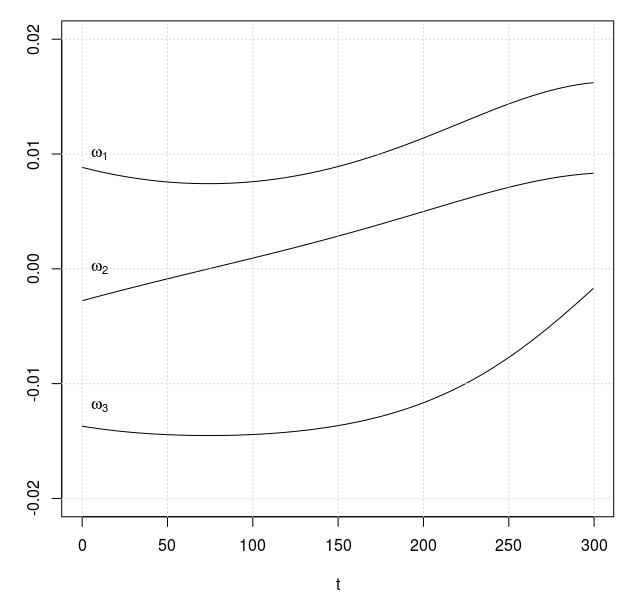
\includegraphics[width=17cm, height=17cm]{o300.png}

Рисунок $2.5$. 
\end{center}


\begin{center}
\vspace*{50px}
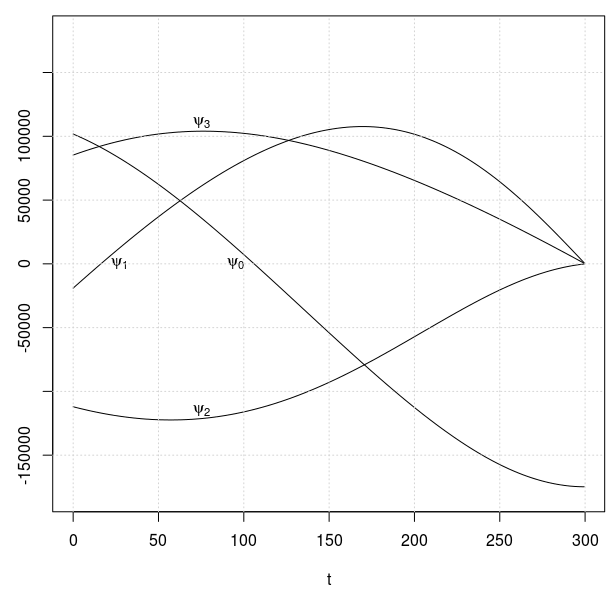
\includegraphics[width=17cm, height=17cm]{p300.png}

Рисунок $2.6$. 
\end{center}

\conclusions

В предоставленной дипломной работе удалось решить задачу оптимального управления углового движения искусственного спутника Земли, 
для которой требовалось составить и решить краевую задачу с помошью принципа максимума Л.С. Понтрягина. 

Были рассмотрены различные поведения системы при различных параметрах. Также удалось программно реализовать алгоритм численного решения задачи
с применением алгебры кватернионов.

Полученные в работе теоритические результаты позволяют понять основные зависимости функционала качества управления и его параметров,
а также прогнозировать поведение системы при изменениях параметров самой задачи.

\begin{thebibliography}{9}
\bibitem{Chelnokov:2006:Kvat_Bikvat} 
Челноков, Ю. Н.
\textit{Кватернионные и бикватернионные модели и методы механики твёрдого тела и их приложения}. 
М.: Физматлит, 2006. – 512c.
 
\bibitem{Branetz_Shmyglevsky:1973:Prim_Kvat_orient} 
Бранец, В. Н., and Шмыглевский, И. П.
\textit{Применение кватернионов в задачах ориентации твердого тела}. 
М.: Наука, 1973. – 320c.

\bibitem{Pontryagin:1983:Matem_theory} 
Понтрягин, Л. С., and Болтянский, В. Г. and Гамкрелидзе, Р. В. and  Мищенко, Е. Ф.
\textit{Математическая теория оптимальных процессов}. 
М.: Наука, 1983 – 393c.

\bibitem{Sapunkov:2001:Chisl_issl_SAU} 
Сапунков, Я. Г.
\textit{Численное исследование систем автоматического управления}. 
М.: Наука, 2001. – 24c.	
	
\bibitem{Gorelov} 
Ю.Н. Горелов
\textit{ЧИСЛЕННЫЕ МЕТОДЫ РЕШЕНИЯ ОБЫКНОВЕННЫХ ДИФФЕРЕНЦИАЛЬНЫХ УРАВНЕНИЙ (МЕТОД РУНГЕ – КУТТА)}. 
Изд-во «Самарский университет», 2006. – 48 с.		

\bibitem{A.S.Antipova, V.G.Birukov} 
А.С. Антипова, Б.Г. Бирюков
\textit{Аналитическое и численное исследование  кинематической задачи оптимальной переориентации твердого тела}. 
УДК – 48 с.	

\bibitem{V.S. Aslanov} 
В. С. Асланов.
\textit{Динамика твёрдого тела и систем тел}. 
Самарский государственный аэрокосмический университет, 2011  – 216с.

\bibitem{Tarasov} 
Тарасов В.Н., Бахарева Н.Ф. 
\textit{Численные методы. Теория, алгоритмы, программы.}. 
Оренбург: ИПК ОГУ, 2008. – 264 с. 

\bibitem{Ermolin} 
Ермолин В. С., Королев В. С., Потоцкая Е. Ю.
\textit{Теоретическая механика. Часть I. Кинематика. Учебное пособие.}. 
СПб: СПбГУ, ВВМ, 2013.— 225 с. 

\bibitem{Telyakovskiy} 
С. А. Теляковский
\textit{Курс лекций по математическому анализу}. 
М.: МИАН, 2009. – 212 с.

\bibitem{Panteleev} 
Пантелеев А.В., Бортаковский А.С., Летова Т.А.
\textit{Оптимальное управление в примерах и задачах.}. 
М: Издательство МАИ, 1996. — 583 с. 

\bibitem{knuthwebsite} 
Knuth: Computers and Typesetting,
\\\texttt{\small{http://www-cs-faculty.stanford.edu/\~{}uno/abcde.html}}

\bibitem{Page11gauss.pdf} 
Прямые методы решения линейных систем
\\\texttt{\small{http://www.math.spbu.ru/user/pan/Page11-gauss.pdf}}

\bibitem{info00036.htm} 
Метод Гаусса
\\\texttt{\small{http://pedsovet.info/info/pages/referats/info\_00036.htm}}

\bibitem{Euler_angles} 
Углы Эйлера
\\\texttt{\footnotesize {https://ru.wikipedia.org/wiki/\%D0\%A3\%D0\%B3\%D0\%BB\%D1\%8B\_\%D0\%AD\%D0\%B9\%D0\%BB\%D0\%B5\%D1\%80\%D0\%B0}}

\bibitem{Conversion_between_quaternions_and_Euler_angles} 
Conversion between quaternions and Euler angles
\\\texttt{\small{http://en.wikipedia.org/wiki/Conversion\_between\_quaternions\_and\_Euler\_angles}}

\bibitem{Newton's method} 
Newton's method
\\\texttt{\small{https://en.wikipedia.org/wiki/Newton\%27s\_method}}

\bibitem{Newton's method} 
Java Platform, Standard Edition (Java SE) 8
\\\texttt{\small{https://docs.oracle.com/javase/8/}}

\bibitem{What Is an Interface?} 
Java: What Is an Interface?
\\\texttt{\small{https://docs.oracle.com/javase/tutorial/java/concepts/interface.html}}

\bibitem{What Is an Interface?} 
R: Documentation
\\\texttt{\small{https://www.r-project.org/other-docs.html}}

\bibitem{What Is an Interface?} 
Исходный код программы
\\\texttt{\small{https://bitbucket.org/guseyn/diploma/src}}

\bibitem{What Is an Interface?} 
Block diagram
\\\texttt{\small{https://en.wikipedia.org/wiki/Block\_diagram}}


\end{thebibliography}

\end{document}
